\documentclass[10pt]{article}
\usepackage{amsmath}
\usepackage{setspace}
\usepackage{hyperref}
\usepackage[pdftex]{graphicx}

\setlength{\textheight}{9in} \setlength{\topmargin}{-.5in}
\setlength{\textwidth}{6.5in} \setlength{\oddsidemargin}{0in}
\setlength{\evensidemargin}{0in}

\title{COMP220 --- Code::Blocks and the StanfordCPPLib}
\author{ }
\date{Fall 2016}

\begin{document}
\maketitle

\begin{abstract}
This documents walks you through the process of building the StanfordCPP library and integrating it with C::B projects. At the time of writing this document the graphics-based components of the library (console.h and obviously graphical libraries) do not work on the server.
\end{abstract}

\section{ Libraries Revisited }

To use a library we must \textit{\#include} the header in the file in which we plan to use the library. This will cause cause the compiler to find the appropriate header and use it to build our object file. The linker then links our object with the library's object to build the executable. This all means that the compiler and linker must know the locations of the library header and object files.

The standard C++ libraries like \textit{iostream} are placed on the server in locations that the compiler and linker know to search. Finding these files requires no intervention on our part. We tip the compiler off a bit by surrounding the library name with $<$ and $>$ rather than quotes, but for the most part the search for standard headers and objects requires no real intervention by the programer.

When we develop our own libraries for use in a project and \#include them by surrounding the name with quotes, we're tipping off the compiler and linker to the fact that the files it needs are in the working directory.  Generally, files in our working directory don't require intervention in order for the compiler and linker to find them.

The Google testing libraries are installed in the usual places so the compiler has no problem resolving the include at the compiler level. However, the gTest libraries are not standard C++ libraries so we must explicitly include link options for their compiled objects. This is the first example we have seen where we the programmer must direct the compiler or linker towards library code we wish to use.


The problem we face with the StanfordCPPLib used by the text is that it is neither standard nor installed on the system. We're given the raw source code for the library and we must incorporate that code into our code. Once we've compiled the project it would be possible to copy the headers and objects into each project's working directory but this is tedious and problematic in the long run. What if we need or want to update the the library? Would we then copy the new files to all the projects that use them? What we need to figure out is how to direct our compiler and linker to libraries that exist outside the usual places.


\section{ Building StanfordCPPLib }

The StanfordCPP Library, like many open source projects, comes with a Makefile setup to build the compiled objects and executables that come with the project. When you build the library you not only get all the objects that we need, but you get an executable program that tests those libraries on your current system. This too is typical as users compiling from source need to be certain that their newly compiled code plays nice with the rest of the system. Let's just walk through the steps:

\begin{enumerate}
\item Copy \textit{stanfordcpplib.zip} from the course home directory to your home directory.
\item From your home directory (or wherever you copied the library zip file to) use the following command sequence to unzip the zip file and change the name of the resultant directory to \textit{stanfordcpplib}
\begin{verbatim}
unzip stanfordcpplib.zip
mv cpplib stanfordcpplib
\end{verbatim}
There should now have the directory stanfordcpplib which contains the contents of the zip file.
\item Change directory to \textit{stanfordcpplib} and run the command \textit{make}. This will compile the library.
\item If compilation succeeds, then run the executable \textit{TestStanfordCPPLib}. It should list a series of success messages like this:
\vspace{.1in}
\begin{center}
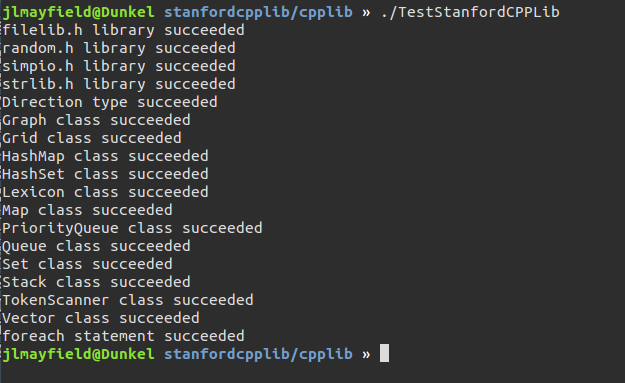
\includegraphics[scale=.5]{scpplib-testspassed.png}
\end{center}
\vspace{.1in}


\end{enumerate}

Assuming no errors compiling or testing, you now have a compiled version of the StanfordCPPLib. The stuff we need is as follows:
\begin{itemize}
\item The \textit{include} directory contains the header files
\item The \textit{obj} directory contains objects
\item The \textit{lib} directory contains the linkable library \textit{libStanfordCPPLib.a}. Check out this description of o type files vs a type files. \url{https://stackoverflow.com/questions/654713/o-files-vs-a-files}
\end{itemize}
Make a mental note of these items and directories as they're the things we need to integrate into C::B.

\section{ Setting up the Build Options }

We'll work on the assumption that every one of our C::B builds needs to include and link to the StanfordCPP library. This means we want to set some global project compiler options. To do this we go to our old friend \textit{Project $>$ Build Options\ldots}.
\begin{enumerate}
\item Go to the \textit{Build Options\ldots} menu
\item Rather than select a specific build from the list, select the project name above the build names. It should be highlighted now, like this:

\vspace{.1in}
\begin{center}
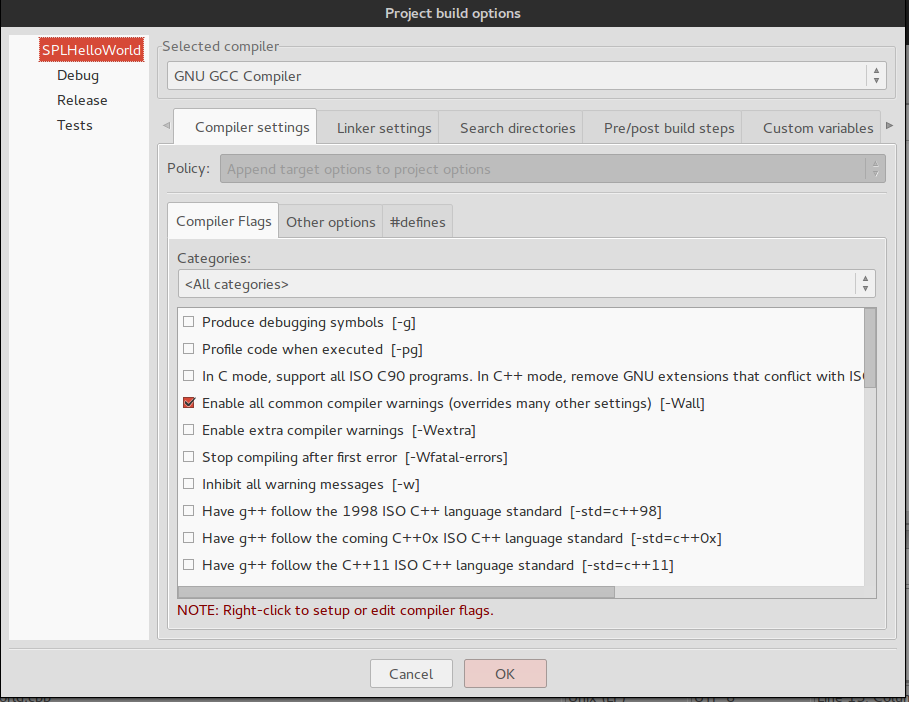
\includegraphics[scale=.4]{buildOpts-proj.png}
\end{center}
\vspace{.1in}

\item Add an \textit{Other Options} to the compiler, namely \textit{-fvisibility-inlines-hidden}

\vspace{.1in}
\begin{center}
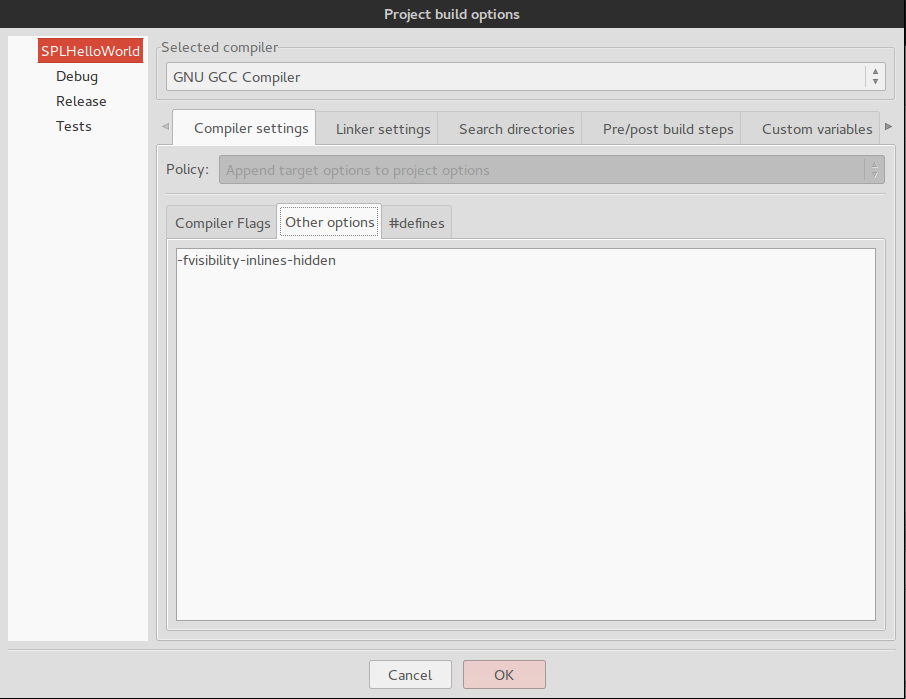
\includegraphics[scale=.4]{scpplib-compopts.png}
\end{center}
\vspace{.1in}

\item Now add an option to the linker to link to \textit{static-libstdc++}and link in \textit{libStanfordCPPLib.a}.  To link the compiled librar (the a type file) you select the \textit{Add} button then direct the file browser to the file.  When asked about relative paths select \textit{No}, we'll do absolute paths for all of this.

\vspace{.1in}
\begin{center}
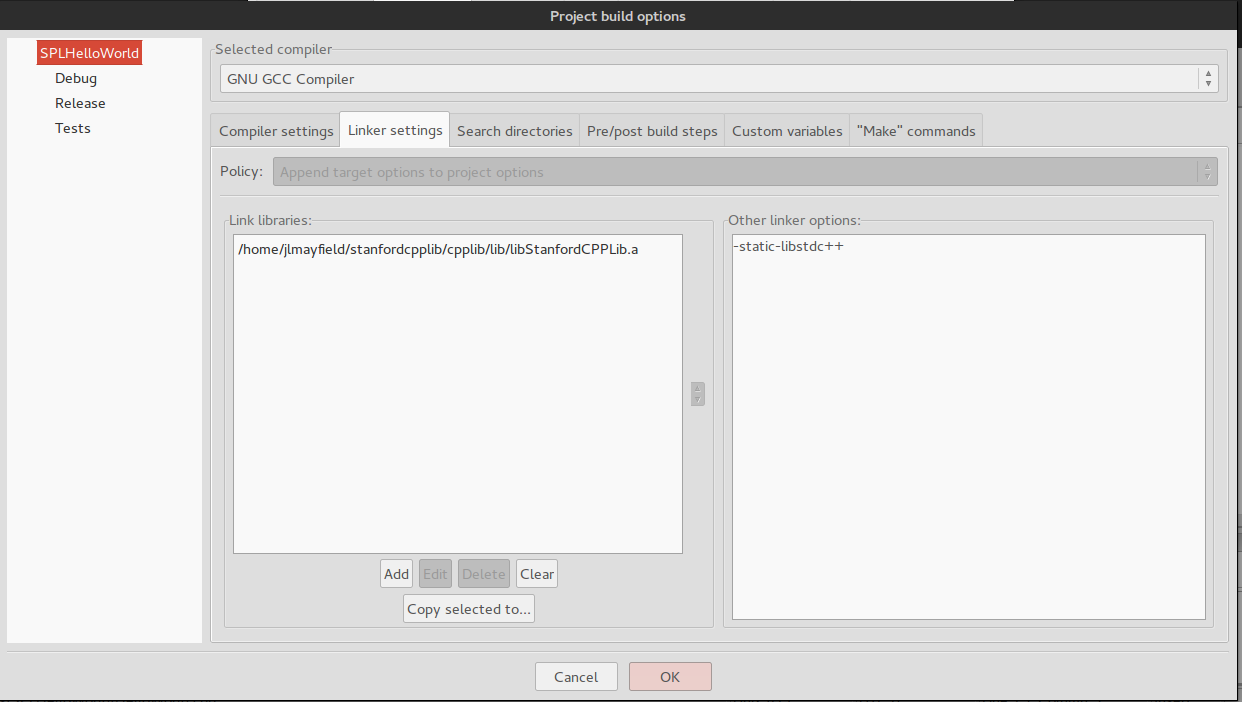
\includegraphics[scale=.35]{scpplib-linker.png}
\end{center}
\vspace{.1in}

\item Now set the compiler search path to include the \textit{include} directory for the library. Once again, use the \textit{Add} button and say No to relative paths.

\vspace{.1in}
\begin{center}
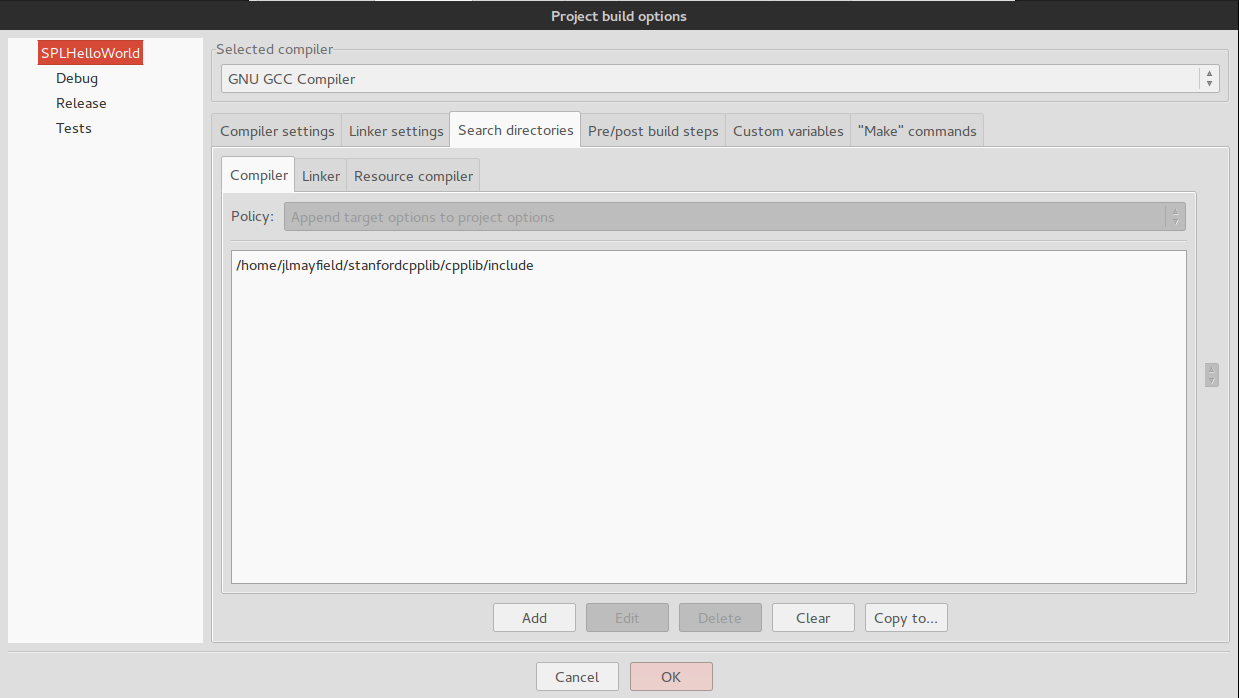
\includegraphics[scale=.35]{scpplib-compilersearch.png}
\end{center}
\vspace{.1in}

\item Now set the linker search path to include the \textit{lib} directory for the library. Once again, use the \textit{Add} button and say No to relative paths.

\vspace{.1in}
\begin{center}
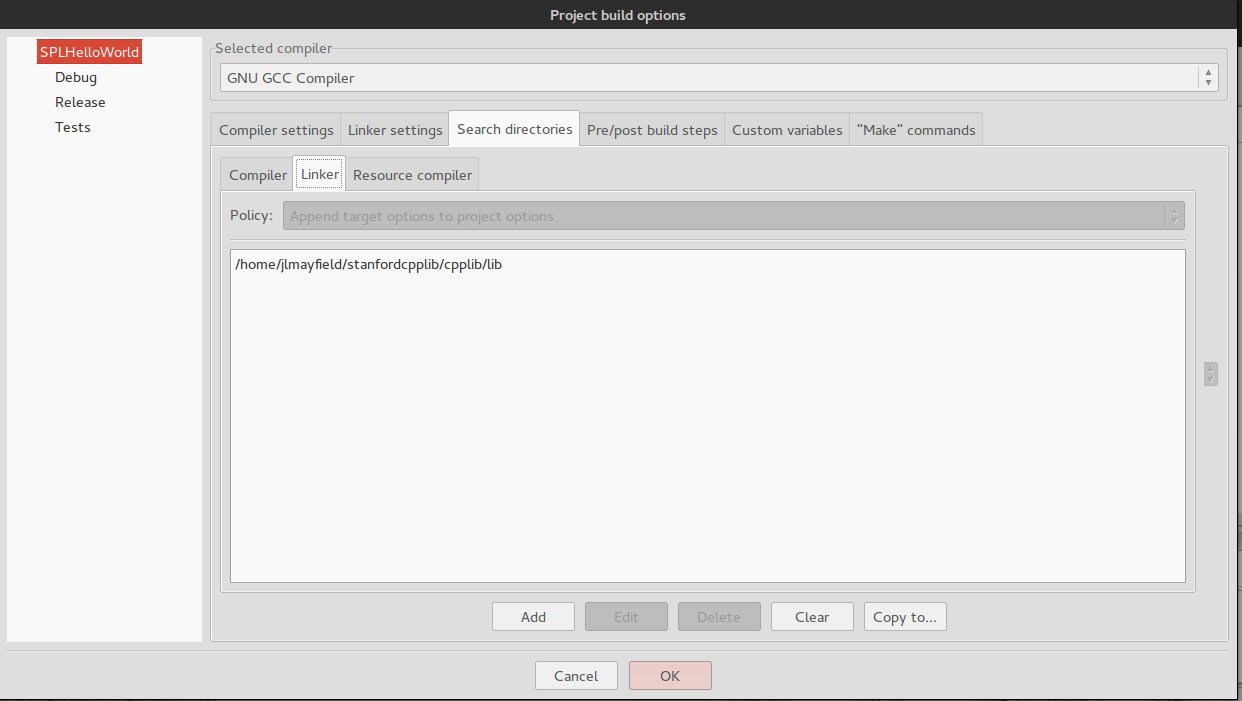
\includegraphics[scale=.35]{scpplib-linkersearch.png}
\end{center}
\vspace{.1in}

\end{enumerate}

At this point your project should be all setup to utilize the StanfordCPP Library. To test it you should write a quick toy program that utilizes some code from the library. There is not shortage of such code in the textbook.


\end{document}
